%!TEX root = paper.tex
%%%%%%%%%%%%%%%%%%%%%%%%%%%%%%%%%%%%%%%%%%%%%%%%%%%%%%%%%%%%%%%%%%%%%%%%%%%%%%%%
\section{Overwatch Lag Simulation}
\label{sec:simulation}

\begin{figure}
	\centering
	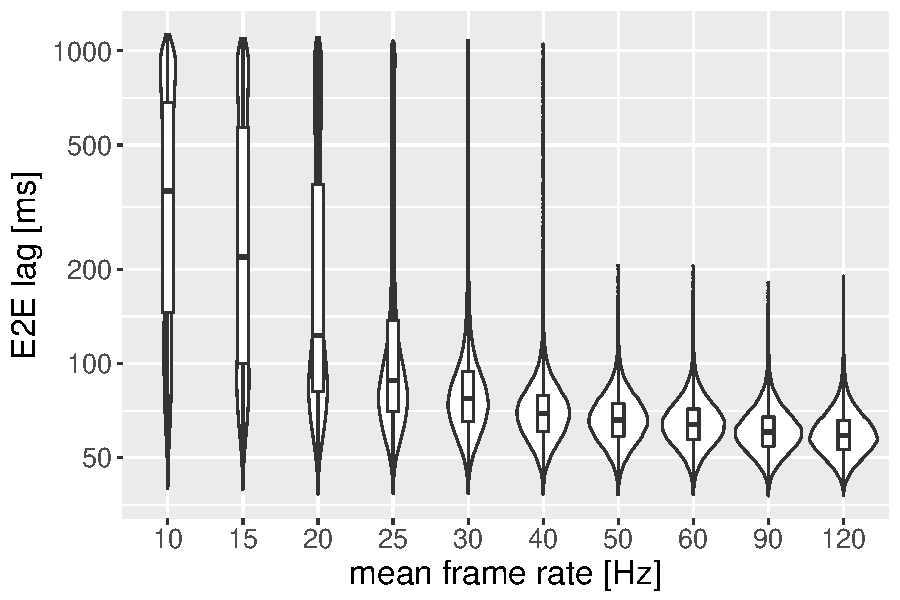
\includegraphics[width=1.0\columnwidth]{images/lagsim.pdf}
	\caption{\acrshort{E2E} lag results of a frame rate study using the \textsc{Overwatch} simulation.}
\label{fig:lagsim}
\end{figure}

Now that all client-observable parameters have been examined, a simulation study is performed on the effects of the game's frame rate. This is more or less the only parameter that the player can influence through the game's setting or through better performing hardware. But since, it is often tricky to maintain a stable frame rate in such resource constrained environments, the target frame rate is just assumed to be the mean of a normal distribution instead of a fixed value. This should account for the variations in the frame times (the time between two consecutive frames). Investigated here were frame rates between \SI{10}{\hertz} and \SI{120}{\hertz}, with the former an unrealistically low value, that nonetheless might occur in high stress situations when resource constraint, and the latter being on the upper end of what modern PC monitors can still display (current models reach roughly \SI{165}{\hertz}). All other simulation parameters are derived from the models in the previous section or left as-is in the base simulation. The results are depicted in Fig.~\ref{fig:lagsim}. Starting at about \SI{50}{\hertz} the \gls{E2E} lag reduction sees diminishing returns especially towards its outliers which can exceed a lag of over a second below \SI{50}{\hertz}. This correlates quite well with the generally accepted notion that (especially) online first person shooters require at least \SI{60}{\hertz} for an enjoyable experience. In praxis, only \SI{30}{\hertz}, \SI{60}{\hertz} or higher frame rates will be targeted due to otherwise occurring issues with the monitor's refresh rate and resulting screen tearing or uneven frame times.





% Server Delay (Bearbeitungszeit des Servers) übernommen als Normalverteilung aus Ursprünglicher Simulation
% - Frames: Normmalverteilung mit mittlerer Framerate von 60 Hz (evtl. Parameterstudie über mittelwert?)
